\section{Hashing}

Molte operazioni richiedono un insieme dinamico che supporta soltanto le operazioni di dizionario \textit{INSERT}, \textit{SEARCH} e \textit{DELETE}. Una \textbf{tavola hash} è una struttura dati efficace per implementare i \textbf{dizionari}. Sebbene la ricerca di un elemento in una tavola hash richieda, nel caso peggiore, lo stesso tempo $\Theta(n)$ richiesto per cercare un elemento in una lista concatenata, l'hashing si comporta molto bene nella pratica. Sotto ipotesi ragionevoli, il tempo medio per cercare un elemento in una tavola hash è $O(1)$.
Una tavola hash è una generalizzazione della nozione più semplice di array ordinario. Quando il numero di \textbf{chiavi} effettivamente memorizzate è piccolo rispetto al numero totale di chiavi possibili, le tavole hash diventano una valida alternativa all'indirizzamento diretto di un array, in quanto una tavola hash tipicamente usa un array di dimensione proporzionale al numero di chiavi effettivamente memorizzate.

\subsection{Tavole a indirizzamento diretto}

L'indirizzamento diretto è una tecnica semplice che funziona bene quando l'universo $U$ delle chiavi è ragionevolmente \textbf{piccolo}. 
Per rappresentare l'insieme dinamico, utilizziamo un array o \textbf{tavola a indirizzamento diretto}, che indicheremo con $T[0...m-1]$, dove ogni posizione o \textbf{cella} corrisponde a una chiave nell'universo $U$. La cella $k$ punta ad un elemento dell'insieme con chiave $k$. Se l'insieme non contiene l'elemento con chiave $k$, allora $T[k]=nil$.

\begin{figure}[htpd]
\centering
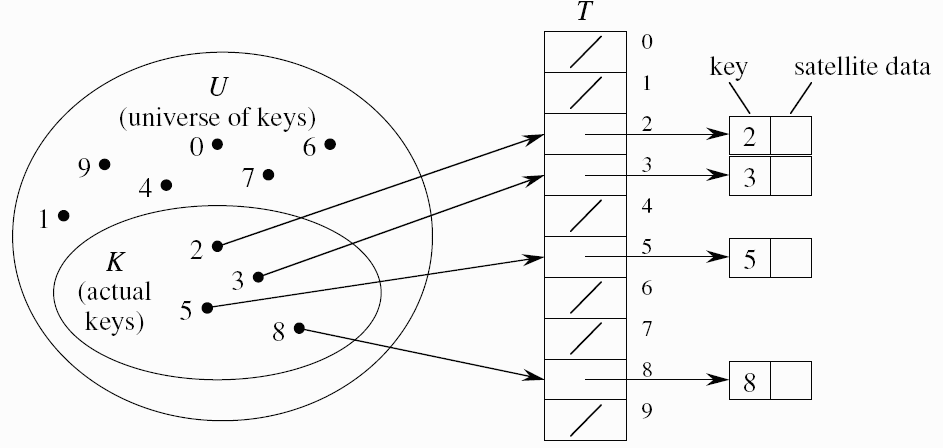
\includegraphics[width=100mm]{images/direct-hash.png}
\caption{Tavola a indirizzamento diretto}
\end{figure}

\begin{lstlisting}

DIRECT-ADDRESS-SEARCH (T, k)
	return T[k]

\end{lstlisting}

\begin{lstlisting}

DIRECT-ADDRESS-INSERT (T,x)
	T[x.key] = x

\end{lstlisting}

\begin{lstlisting}

DIRECT-ADDRESS-DELETE (T, x)
	T[x.key] = nil

\end{lstlisting}

Ciascuna di queste operazioni richiede tempo $O(1)$.

\subsection{Tavole hash}

La difficoltà dell'indirizzamento diretto è ovvia: se l'universo $U$ delle chiavi è troppo grande, memorizzare una tavola $T$ di dimensione $|U|$ può essere impraticabile. Inoltre, l'insieme $K$ delle chiavi \textit{effettivamente memorizzate} può essere così piccolo rispetto a $U$ che la maggior parte dello spazio allocato per la tavola $T$ sarebbe sprecato.

Con l'indirizzamento diretto un elemento con chiave $k$ è memorizzato nella cella $k$. Con l'hashing, questo elemento è memorizzato nella cella $h(k)$: cioè utilizziamo una \textbf{funzione hash} $h$ per calcolare la cella dalla chiave $k$. Qui $h$ associa l'universo $U$ delle chiavi alle celle di una \textbf{tavola hash} $T[0...m-1]$:

$$h:U\to \{0,1,...,m-1\}$$

dove la dimensione $m$ della tavola hash è generalmente molto più piccola di $|U|$. Diciamo che un elemento con chiave $k$ viene mappato nella cella $h(k)$ o anche che $h(k)$ è il \textbf{valore hash} della chiave $k$.

Il compito della funzione hash è quello di ridurre l'intervallo degli indici e di conseguenza la dimensione dell'array. L'array ha dimensione $m$ invece di $|U|$.

\begin{figure}[htpd]
\centering
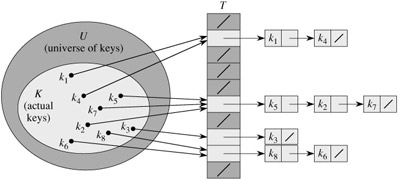
\includegraphics[width=100mm]{images/hashing.jpg}
\caption{Utilizzo di una funzione hash}
\end{figure}

C'è un problema: due chiavi possono essere mappate nella stessa cella. Questo evento si chiama \textbf{collisione}. Fortunatamente ci sono tecniche efficaci per risolvere i conflitti creati dalle collisioni.

\subsubsection{Risoluzione delle collisioni mediante concatenamento}

Nel \textbf{concatenamento} poniamo tutti gli elementi che sono associati alla stessa cella in una lista concatenata. La cella contiene un puntatore alla testa della lista di tutti gli elementi memorizzati che vengono mappati in $j$; se non ce ne sono, la cella $j$ contiene la costante $nil$. Le operazioni di dizionario sono facili da implementare:

\begin{lstlisting}

CHAINED-HASH-INSERT (T, x)
	inserisce x in testa alla lista T[h(x.key)]

\end{lstlisting}

\begin{lstlisting}

CHAINED-HASH-SEARCH (T, x)
	ricerca un elemento con chiave k nella lista T[h(k)]

\end{lstlisting}

\begin{lstlisting}

CHAINED-HASH-DELETE (T, x)
	cancella x dalla lista T[h(x.key)]

\end{lstlisting}

Il tempo di esecuzione nel caso peggiore per l'inserimento è $O(1)$.

\subsubsection{Analisi dell'hashing con concatenamento}

Data una tavola hash $T$ con $m$ celle dove sono memorizzati $n$ elementi, definiamo \textbf{fattore di carico} $\alpha$ della tavola $T$ il rapporto $n/m$, ossia il numero medio di elementi memorizzati in una lista.

Il comportamento nel caso peggiore dell'hashing con concatenamento è pessimo: tutte le $n$ chiavi sono associate alla stessa cella, creando una lista di lunghezza $n$. Il tempo di esecuzione della ricerca è quindi $\Theta(n)$, più il tempo per calcolare la funzione hash.

Le prestazioni dell'hashing nel caso medio dipendono dal modo in cui la funzione hash $h$ distribuisce mediamente l'insieme delle chiavi da memorizzare tra le $m$ celle. Per adesso supponiamo che qualsiasi elemento abbia la stessa probabilità di essere mandato in una qualsiasi delle $m$ celle, indipendentemente dalle celle in cui sono mandati gli altri elementi. Questa ipotesi è detta \textbf{hashing uniforme semplice}.

\subsubsection*{Teorema}

In una tavola hash le cui collisioni sono risolte con il concatenamento, una ricerca senza successo richiede un tempo $\Theta(1+\alpha)$ nel caso medio, nell'ipotesi di hashing uniforme semplice.

\subsubsection*{Teorema}

In una tavola hash le cui collisioni sono risolte con il concatenamento, una ricerca con successo richiede un tempo $\Theta(1+\alpha)$ nel caso medio, nell'ipotesi di hashing uniforme semplice
\linebreak
\linebreak
Se il numero di celle della tavola hash è almeno proporzionale al numero di elementi della tavola, abbiamo $n = O(m)$ e, di conseguenza, $\alpha=n/m=O(m)/m=O(1)$ nel caso peggiore e la cancellazione richiede il tempo $O(1)$ nel caso peggiore quando le liste sono doppiamente concatenate, tutte le operazioni di dizionario possono essere svolte, in media, nel tempo $O(1)$.

\subsection{Funzioni hash}

Una buona funzione hash soddisfa l'ipotesi dell'hashing uniforme semplice: ogni chiave ha la stessa probabilità di essere mandata in una qualsiasi delle $m$ celle, indipendentemente dalla cella cui viene mandata qualsiasi altra chiave.

Purtroppo, di solito non è possibile verificare questa condizione, in quanto raramente è nota la distribuzione delle probabilità secondo la quale vengono estratte le chiavi. Ad esempio se le chiavi sono numeri reali casuali $k$ distribuiti in modo indipendente e uniforme nell'intervallo $0\le k < 1$, la funzione hash:

$$h(k)=\floor*{km}$$

soddisfa la condizione dell'hashing uniforme semplice.

La maggior parte delle funzioni hash suppone che l'universo delle chiavi sia l'insieme dei numeri naturali: $\mathbb{N}=\{0,1,2,...\}$. Quindi se le chiavi non sono numeri naturali, occorre un metodo per interpretarle come tali.

\subsubsection{Il metodo della divisione}

Quando si applica il \textbf{metodo della divisione} per creare una funzione hash, una chiave $k$ viene associata ad una delle $m$ celle prendendo il resto della divisione fra $k$ ed $m$, cioè la funzione hash è:

$$h(k)=k\mod m$$

Un numero primo non troppo vicino a una potenza esatta di 2 è spesso una buona scelta per $m$. Per esempio supponiamo di allocare una tavola hash per contenere circa $n=2000$ stringhe di caratteri, dove ogni carattere ha 8 bit. Poichè riteniamo accettabile esaminare in media 3 elementi in una ricerca senza successo, allochiamo una tavola hash di dimensione $m=701$. Abbiamo scelto 701 perchè è un numero primo vicino a 2000/3, ma non a una potenza di 2. Trattando ogni chiave $k$ come un numero intero, la funzione hash diventa:

$$h(k)=k\mod 701$$

\subsubsection{Il metodo della moltiplicazione}

Il \textbf{metodo della moltiplicazione} per creare funzioni hash si svolge in due passi. Prima moltiplichiamo la chiave $k$ per una costante $A$ nell'intervallo $0<A<1$ ed estraiamo la parte frazionaria di $kA$. Poi moltiplichiamo questo valore per $m$ e prendiamo la parte intera inferiore del risultato. In sintesi la funzione hash è:

$$h(k)=\floor*{m(kA\mod 1)}$$

Un vantaggio del metodo di moltiplicazione è che non è critico. Tipicamente, lo scegliamo come una potenza di 2 ($m=2^p$ per qualche intero $p$), il che rende semplice implementare la funzione hash nella maggior parte dei calcolatori.

\subsection{Indirizzamento aperto}

Nell'\textbf{indirizzamento aperto}, tutti gli elementi sono memorizzati nella tavola hash stessa; ovvero ogni cella della tavola contiene un elemento dell'insieme dinamico o la costante $nil$. Quando cerchiamo un elemento, esaminiamo sistematicamente le celle della tavola finchè non troviamo l'elemento desiderato o finchè non ci accorgiamo che l'elemento non si trova nella tavola.s

Diversamente dal concatenamento non ci sono nè liste nè elementi memorizzati all'esterno della tavola, quindi la tavola può ``riempirsi'' al punto tale che non possono essere effettuati altri inserimenti. Una conseguenza è che il fattore di carico $\alpha$ non supera mai 1.

Il vantaggio dell'indirizzamento aperto sta nel fatto che esclude completamente i puntatori. Anzichè seguire i puntatori, \textit{calcoliamo} la sequenza delle celle da esaminare. La memoria extra liberata per non aver memorizzato i puntatori offre alla tavola hash un maggior numero di celle, a parità di memoria occupata, consentendo potenzialmente di ridurre il numero di collisioni e di accelerare le operazioni di ricerca.

Per effettuare un inserimento mediante l'indirizzamento aperto, esaminiamo in successione le posizioni della tavola hash (\textbf{ispezione}), finchè non troviamo una cella vuota in cui inserire la chiave. La sequenza delle posizioni esaminate durante un'ispezione \textit{dipende dalla chiave da inserire}.

Con l'indirizzamento aperto si richiede che, per ogni chiave $k$, la \textbf{sequenza di ispezione}:

$$\langle h(k,0),h(k,1),...,h(k,m-1)\rangle$$

sia una permutazione di $\langle 0,1,...,m-1\rangle$, in modo che ogni posizione della tavola hash possa essere considerata come possibile cella in cui inserire una nuova chiave mentre la chiave si riempe.

\subsubsection{Ispezione lineare}

Data una funzione hash ordinaria $h':U\to \{0,1,...,m-1\}$, che chiameremo \textbf{funzione hash ausiliaria}, il metodo dell'\textbf{ispezione lineare} usa la funzione hash:

$$h(k,i)=(h'(k)+i)\mod m$$

per $i=0,1,...,m-1$.

L'ispezione lineare è facile da implementare, ma presenta un problema noto come \textbf{addensamento primario}: si formano lunghe file di celle occupate, che aumentano il tempo medio di ricerca.

\subsubsection{Ispezione quadratica}

L'\textbf{ispezione quadratica} usa una funzione hash della forma:

$$h(k,i)=(h'(k)+c_1i+c_2i^2)\mod m$$

dove $h'$ è una funzione hash ausiliaria, $c_1$ e $c_2\neq 0$ sono costanti ausiliarie e $i=0,1,...,m-1$. La posizione iniziale esaminata è $T[h'(k)]$; le posizioni successivamente esaminate sono distanziate da quantità che dipendono in modo quadratico dal numero di ispezione $i$. Questa tecnica funziona molto meglio dell'ispezione lineare, ma per fare pieno uso della tavola hash, i valori di $c_1$, $c_2$ ed $m$ non si possono scegliere arbitrariamente.

\subsubsection{Doppio hashing}

Il doppio hashing è uno dei metodo migliori disponibili per l'indirizzamento aperto, perchè le permutazioni prodotte hanno molte delle caratteristiche delle permutazioni scelte a caso. Il \textbf{doppio hashing} usa una funzione hash della forma:

$$h(k,i)=(h_1(k)+ih_2(k))\mod m$$

dove $h_1$ e $h_2$ sono funzioni hash ausiliarie. L'ispezione inizia dalla posizione $T[h_1(k)]$; le successive posizioni sono distanziate dalle precedenti posizioni di una quantità $h_2(k)$, modulo $m$. Quindi, diversamente dal caso dell'ispezione linare o quadratica, la sequenza di ispezione qui dipende in due modi dalla chiave $k$, perchè possono variare sia la posizione iniziale di ispezione sia la distanza fra due posizioni successive di ispezione.

Il valore $h_2(k)$ dev'essere relativamente primo con la dimensione $m$ della tavola hash perchè venga ispezionata l'intera tavola hash. Un modo pratico per garantire questa condizione è scegliere $m$ potenza di 2 e definire $h_2$ in modo che produca sempre un numero dispari.

\subsection{Domande}

\subsubsection*{Domanda 1}

Spiegare cos'è l'ipotesi di hash uniforme semplice. Come bisogna scegliere la funzione hash perchè tale ipotesi sia soddisfatta?
\linebreak
\linebreak
\textbf{Risposta}: l'ipotesi di hash uniforme semplice assume che una chiave da inserire nella tavola abbia uguale probabilità di finire in una qualsiasi delle celle della tavola, indipendentemente dalle chiavi inserite precedentemente. Poichè sia soddisfatta tale ipotesi, occorre scegliere la funzione hash tenendo conto della distribuzione di probabilità delle chiavi in input. Alternativamente possiamo scegliere casualmente la funzione hash in un insieme universale.

\subsubsection*{Domanda 2}

Sia $h(k)$ una funzione hash che mappa un insieme $U$ di chiavi in una tavola hash di $m$ celle. Mostrare che esiste una cella in cui la funzione hash manda almeno $\ceil{|U|/m}$ chiavi distinte.
\linebreak
\linebreak
\textbf{Risposta}: se la funzione hash $h(k)$ mandasse al più $\ceil{|U|/m}-1$ chiavi, in ogni cella dovremmo avere al massimo $m(\ceil{|U|/m})$ chiavi. Sia $|U|=qm+r$, con $q$ ed $r$ quoziente e resto della divisione per $m$. Se $r=0$ allora $m(\ceil{|U|/m}-1)=|U|-1<|U|$: assurdo. Se $r>0$ allora $m(\ceil{|U|/m}-1)=mq<|U|$: assurdo. Deve quindi esistere almeno una cella in cui la funzione hash $h(k)$ manda almeno $\ceil{|U|/m}$ chiavi.

\subsubsection*{Domanda 3}

Una tavola hash con risoluzione delle collisioni mediante liste, usa la funzione hash $h(k)=k\mod 257$. Tale tavola hash viene usata per memorizzare delle stringhe di caratteri ASCII. Mostrare che se la stringa $y$ è ottenuta dalla stringa $x$ permutandone i caratteri di posto pari allora $x$ ed $y$ vengono messe nella stessa cella.
\linebreak
\linebreak
\textbf{Risposta}: siccome $256\mod 257 \equiv 1$ e quindi $256^i\mod 257 \equiv (-1)^i$ abbiamo che:

$$h(k)=k\mod 257=(\sum_{i=0}^nc_i(-1)^i)\mod 257=$$
$$=(\sum_{i=0}^nc_i(-1)^i)\mod 257$$

I caratteri di posto pari risultano tutti moltiplicati per 1 e quindi per la commutatività della somma, permutandoli tra loro non cambia il valore di $h(k)$.

\subsubsection*{Domanda 4}

Dire perchè in una tavola hash con indirizzamento aperto non è possibile eliminare un elemento ponendo il valore $nil$ nella cella ma occorre introdurre un nuovo valore $deleted$ diverso sia da $nil$ che da ogni chiave.
\linebreak
\linebreak
\textbf{Risposta}: Se l'elemento eliminato non è l'ultimo elemento della sequenza di ispezione a cui esso appartiene, ponendo il valore a $nil$ nella cella la ricerca degli elementi successivi (che non sono stati rimossi) si ferma non appena trova il valore $nil$ e dà risultato negativo.

\subsubsection*{Domanda 5}

Spiegare il fenomeno dell'addensamento primario in una tavola hash con indirizzamento aperto e che usa l'ispezione lineare.
\linebreak
\linebreak
\textbf{Risposta}: L'ispezione lineare usa la funzione hash:

$$h(k,i)=(h'(k)+1)\mod m$$

assumendo che $h'(k)$ soddisfi l'ipotesi di hash uniforme semplice, se la tavola è vuota l'inserimento della prima chiave può avvenire con uguale probabilità $1/m$ in una qualsiasi delle $m$ celle della tavola. Ma essendo la cella $h'(k_1)$ occupata dalla chiave $k_1$, se $h'(k_2)=h'(k_1)$ la chiave $k_2$ viene rimandata nella cella successiva $h'(k_1)+1$. Di conseguenza la probabilità che $k_2$ venga mandata nella cella $h'(K_1)+1$ è doppia, ossia pari a $2/m$. In generale, se una cella libera è preceduta da $n$ celle consecutive occupate, la probabilità che la prossima chiave venga messa in tale cella è pari ad $(n+1)/m$. Di conseguenza sequenze consecutive di celle occupate tendono ad allungarsi sempre di più.

\subsubsection*{Domanda 6}

Come la domanda 1 ma con $h(k)=k\mod 17$, e con $y$ ottenuta da $x$ permutando i caratteri.
\linebreak
\linebreak
\textbf{Risposta}: siccome $256^i\mod 17 = 1$ abbiamo che:

$$h(k)=k\mod 17 = (\sum_{i=0}^nc_i256^i)\mod 17=(\sum_{i=0}^nc_i)\mod 17$$

Per la commutatività della somma, permutando i caratteri non cambia il valore di $h(k)$.

